\section{Loss Functions}
\begin{frame}{Task Type A: Regression}
    \begin{columns}[c]
        % Left: Concept & Math
        \begin{column}{0.53\textwidth}
            \textbf{Definition:}
            The target $y$ is \textbf{Continuous} ($y \in \mathbb{R}$).
            
            \vspace{1em}
            \textbf{Examples:}
            \begin{itemize}
                \item House Prices ($\$300k, \$500k$)
                \item Temperature ($24.5^\circ C$)
                \item Stock Value
            \end{itemize}

            \vspace{1em}
            \begin{tcolorbox}[colback=blue!5, title=The Loss: Mean Squared Error]
                Measures the squared distance between points and the line.
                $$ \text{MSE} = \frac{1}{N} \sum (y - \hat{y})^2 $$
            \end{tcolorbox}
        \end{column}

        % Right: Visual
        \begin{column}{0.5\textwidth}
            \centering
            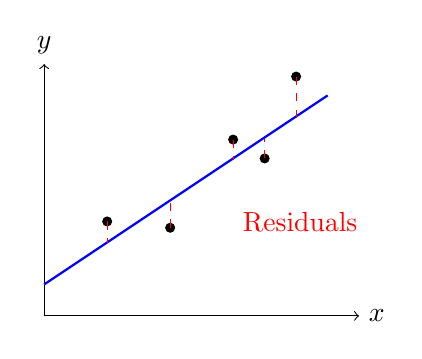
\begin{tikzpicture}[scale=0.8]
                \draw[->] (0,0) -- (5,0) node[right] {$x$};
                \draw[->] (0,0) -- (0,4) node[above] {$y$};
                
                % Regression Line
                \draw[blue, thick] (0,0.5) -- (4.5,3.5);
                
                % Points and Residuals
                \foreach \x/\y in {1/1.5, 2/1.4, 3/2.8, 3.5/2.5, 4/3.8} {
                    \filldraw[black] (\x,\y) circle (2pt);
                    % Calculate point on line y = 0.66x + 0.5
                    \pgfmathsetmacro{\yhat}{0.66*\x + 0.5}
                    \draw[red, dashed] (\x,\y) -- (\x,\yhat);
                }
                \node[red, right] at (3,1.5) {Residuals};
            \end{tikzpicture}
            \vspace{0.5em}
            \small \textit{Goal: Minimize the sum of red lines.}
        \end{column}
    \end{columns}
\end{frame}

\begin{frame}{Why Squared Error?}
    \begin{columns}[T]
        % Left: Step-by-step logic
        \begin{column}{0.55\textwidth}
            \textbf{The 3 Steps to MSE Loss:}
            
            \vspace{0.8em}
            \begin{enumerate}
                \item \textbf{Residuals ($y - \hat{y}$):} measures the raw distance. Points below the line give \textcolor{red}{negative} distances.
                \item \textbf{The Square $(\dots)^2$:} Squaring ensures all distances are positive so they don't cancel out. It also heavily penalizes \textbf{outliers}.
                \item \textbf{The Average ($\frac{1}{N} \sum$):} We aggregate errors from all $N$ samples to get a single performance score.
            \end{enumerate}
        \end{column}

        % Right: Visual Intuition of Squares
        \begin{column}{0.45\textwidth}
            \centering
            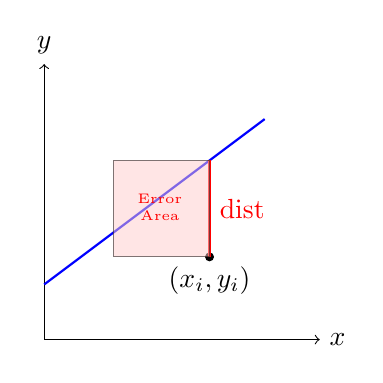
\begin{tikzpicture}[scale=0.7]
                \draw[->] (0,0) -- (5,0) node[right] {$x$};
                \draw[->] (0,0) -- (0,5) node[above] {$y$};
                \draw[blue, thick] (0,1) -- (4,4);
                
                % Example of a 'Square' error
                \filldraw[black] (3,1.5) circle (2pt) node[below] {$(x_i, y_i)$};
                \draw[red, thick] (3,1.5) -- (3,3.25) node[midway, right] {dist};
                
                % Draw a literal square to show "Squared" error
                \draw[fill=red!20, opacity=0.5] (3,1.5) rectangle (1.25, 3.25);
                \node[red, font=\tiny, align=center] at (2.1, 2.4) {Error\\Area};
            \end{tikzpicture}
            \vspace{0.5em}
            \small \textit{Each "error" acts as a square area we want to shrink to zero.}
        \end{column}
    \end{columns}
\end{frame}

\begin{frame}{Why Squared Error?}
    \begin{columns}[T]
        % Left: Step-by-step logic
        \begin{column}{0.55\textwidth}
            \begin{tcolorbox}[colback=blue!5, title=Note]
                If we use the \textbf{Absolute} difference $|y - \hat{y}|$ instead of the square, we get \textbf{MAE}. It is more robust to outliers, but \textbf{not differentiable} at 0. \\
                Mathematically, you can still optimize functions with \textbf{finitely} many non-differentiable points using subgradients, though this adds some complexity.
            \end{tcolorbox}
        \end{column}

        % Right: Visual Comparison (U vs V)
        \begin{column}{0.45\textwidth}
            \centering
            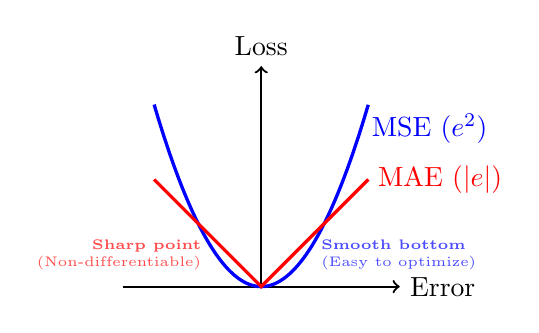
\begin{tikzpicture}[scale=0.8]
                % Axes
                \draw[->, thick] (-2.2,0) -- (2.2,0) node[right] {Error};
                \draw[->, thick] (0,0) -- (0,3.5) node[above] {Loss};

                % MSE (Parabola) - Blue U-Shape
                \draw[blue, very thick, domain=-1.7:1.7, samples=100] plot (\x, {\x*\x});
                \node[blue, right] at (1.6, 2.5) {MSE ($e^2$)};

                % MAE (Absolute) - Red V-Shape
                \draw[red, very thick] (-1.7, 1.7) -- (0,0) -- (1.7, 1.7);
                \node[red, right] at (1.7, 1.7) {MAE ($|e|$)};

                % Annotations

                \node[right, blue!70, font=\tiny, align=left] at (0.8, 0.5) {\textbf{Smooth bottom}\\(Easy to optimize)};


                \node[left, red!70, font=\tiny, align=right] at (-0.8, 0.5) {\textbf{Sharp point}\\(Non-differentiable)};
            \end{tikzpicture}
            \vspace{0.5em}
            \small \textit{MSE (Blue) is smooth. MAE (Red) is sharp.}
        \end{column}
    \end{columns}
\end{frame}

% Slide 1: Binary Classification Introduction
\begin{frame}{Task Type B: Binary Classification}
    \begin{columns}[c]
        % Left: Concept & Math
        \begin{column}{0.5\textwidth}
            \textbf{Definition:}\\
            Target $y$ is \textbf{discrete}: $y \in \{0, 1\}$ (e.g., spam/not spam)
            
            \vspace{1.2em}
            \textbf{How It Works:}
            \begin{enumerate}
                \item Model outputs \textbf{probability}: $\hat{y} \in [0, 1]$
                \item Apply \textbf{threshold} (usually 0.5) to classify
                \item If $\hat{y} \geq 0.5 \to$ Class 1, else Class 0
            \end{enumerate}
            
            \vspace{0.8em}
            \begin{exampleblock}{Example}
                \centering
                $\hat{y}=0.87 \xrightarrow{\text{threshold } 0.5}$ \textbf{Class 1} (Spam)
            \end{exampleblock}
        \end{column}

        % Right: Visual
        \begin{column}{0.5\textwidth}
            \centering
            \textbf{Decision Boundary Visualization}
            \vspace{0.5em}
            
            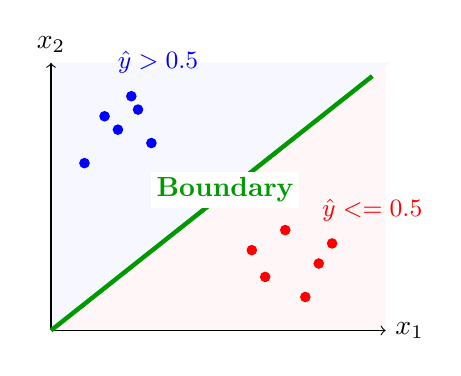
\begin{tikzpicture}[scale=0.85]

            % Shaded regions (draw FIRST) - consistent with boundary (0,0) -- (4.8,3.8)
            \fill[red!10, opacity=0.3] (0,0) -- (5,0) -- (5,4) -- (5.0526,4) -- cycle; % above/left side
            \fill[blue!10,  opacity=0.3] (0,0) -- (5.0526,4) -- (0,4) -- cycle;          % below/right side

        
            % Axes
            \draw[->] (0,0) -- (5,0) node[right] {$x_1$};
            \draw[->] (0,0) -- (0,4) node[above] {$x_2$};
        
            % Decision Boundary (now full)
            \draw[green!60!black, ultra thick] (0,0) -- (4.8,3.8);
            \node[green!60!black, font=\bfseries, fill=white, inner sep=2pt] at (2.6,2.1) {Boundary};
        
            % Classes
            \foreach \x/\y in {0.8/3.2, 1.2/3.5, 1.5/2.8, 0.5/2.5, 1/3, 1.3/3.3}
                \filldraw[blue] (\x, \y) circle (2pt);
        
            \foreach \x/\y in {3/1.2, 3.5/1.5, 4/1, 3.2/0.8, 3.8/0.5, 4.2/1.3}
                \filldraw[red] (\x, \y) circle (2pt);
        
            % Probability labels
            \node[blue, font=\small\bfseries] at (1.6, 4) {$\hat{y} > 0.5$};
            \node[red,  font=\small\bfseries] at (4.8, 1.8) {$\hat{y} <= 0.5$};
        
        \end{tikzpicture}

            
            \vspace{0.5em}
            \small \textit{Goal: Find optimal boundary that maximizes class separation}
        \end{column}
    \end{columns}
\end{frame}



% Slide 2: Motivation - Why Not MSE?
\begin{frame}{Can We Use MSE Loss for Classification?}
    \begin{alertblock}{Problem with MSE}
        MSE measures \textbf{numeric distance}, but in classification, we care about \textbf{probability confidence}, not distance!
    \end{alertblock}

\end{frame}

% Slide 2: Motivation - Why Not MSE?
\begin{frame}{Can We Use MSE Loss for Classification?}
    \begin{alertblock}{Problem with MSE}
        MSE measures \textbf{numeric distance}, but in classification, we care about \textbf{probability confidence}, not distance!
    \end{alertblock}
    
    \vspace{1em}
    
    \begin{alertblock}{What We Really Want}
        A loss function that \textbf{heavily penalizes confident wrong predictions}
        
        \vspace{0.5em}
        \textbf{Example:} Classifying an image as a dog with 98\% confidence when it's actually a cat should incur massive penalty!
    \end{alertblock}
\end{frame}

\subsection{Classification}

% Slide 2: Motivation - Why Not MSE?
\begin{frame}{Can We Use MSE Loss for Classification?}
    \begin{alertblock}{Problem with MSE}
        MSE measures \textbf{numeric distance}, but in classification, we care about \textbf{probability confidence}, not distance!
    \end{alertblock}
    
    \vspace{1em}
    
    \begin{alertblock}{What We Really Want}
        A loss function that \textbf{heavily penalizes confident wrong predictions}
        
        \vspace{0.5em}
        \textbf{Example:} Classifying an image as a dog with 98\% confidence when it's actually a cat should incur massive penalty!
    \end{alertblock}
    
    \vspace{1.5em}
    
    \begin{block}{Solution: The Logarithm!}
        The logarithm function has exactly the property we need:\\
        it grows exponentially as confidence in the \textbf{wrong} class increases
    \end{block}
\end{frame}

% Slide 3: How Logarithm Works
\begin{frame}{The Power of the Logarithm}
    \begin{columns}[T]
        % Left: Intuition
        \begin{column}{0.50\textwidth}
            \textbf{Intuition (True Label $y=1$):}
            \vspace{0.5em}
            
            Model outputs probability $\hat{y}$ for class 1
            
            \vspace{0.5em}
            \textbf{Log Penalty} $= -\log(\hat{y})$ behaves as:
            \begin{itemize}
                \item $\hat{y} = 0.99 \to$ Loss $\approx 0.01$ \textcolor{green!60!black}{\textbf{✓ Great!}}
                \vspace{0.3em}
                \item $\hat{y} = 0.50 \to$ Loss $\approx 0.69$ \textcolor{orange}{\textbf{⚠️ Uncertain}}
                \vspace{0.3em}
                \item $\hat{y} = 0.01 \to$ Loss $\approx 4.6$ \textcolor{red}{\textbf{✗ Disaster!}}
            \end{itemize}
            
            \vspace{1em}
            \begin{tcolorbox}[colback=yellow!10, colframe=orange, boxsep=4pt]
                The same concept applies when the true label is 0.
            \end{tcolorbox}
        \end{column}

        % Right: Visual Curve
        \begin{column}{0.50\textwidth}
            \centering
            \textbf{Loss vs. Predicted Probability}\\
            \vspace{-0.2em}
            \small (when true label = 1)
            \vspace{0.3em}
            
            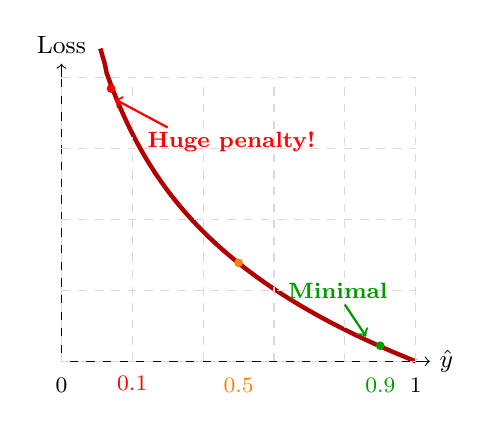
\begin{tikzpicture}[scale=0.9]
                % Axes
                \draw[->] (0,0) -- (5.2,0) node[right, font=\small] {$\hat{y}$};
                \draw[->] (0,0) -- (0,4.2) node[above, font=\small] {Loss};

                % Log Loss Curve
                \draw[red!70!black, ultra thick, domain=0.55:5, samples=150] 
                    plot (\x, {-ln(\x/5)*2});
                
                % Grid lines
                \draw[dashed, gray!30] (0,0) grid[step=1] (5,4);
                
                % Key points
                \filldraw[green!60!black] (4.5, 0.22) circle (1.5pt);
                \node[below, green!60!black, font=\footnotesize] at (4.5, -0.1) {0.9};
                
                \filldraw[orange] (2.5, 1.39) circle (1.5pt);
                \node[below, orange, font=\footnotesize] at (2.5, -0.1) {0.5};
                
                \filldraw[red] (0.7, 3.85) circle (1.5pt);
                \node[above right, red, font=\footnotesize] at (0.65, -0.55) {0.1};
                
                % Annotations with arrows
                \draw[->, red, thick] (1.5, 3.3) -- (0.75, 3.7);
                \node[red, font=\footnotesize] at (2.4, 3.1) {\textbf{Huge penalty!}};
                
                \draw[->, green!60!black, thick] (4.0, 0.8) -- (4.3, 0.35);
                \node[green!60!black, font=\footnotesize] at (3.9, 1.0) {\textbf{Minimal}};
                
                % Axis labels
                \node[below, font=\footnotesize] at (0, -0.1) {0};
                \node[below, font=\footnotesize] at (5, -0.1) {1};
            \end{tikzpicture}
            
            \begin{block}{}
                \centering
                \small Curve explodes as $\hat{y} \to 0$\\
                \textbf{Forces model to be cautious!}
            \end{block}
        \end{column}
    \end{columns}
\end{frame}

% Slide 4: Binary Cross-Entropy Formula
\begin{frame}{Binary Cross-Entropy Loss (Log Loss)}
    \begin{tcolorbox}[colback=blue!5, colframe=blue!60, title=\textbf{Loss Function: Binary Cross-Entropy (Log Loss)}]
        $$ J(\mathbf{w}) = - \frac{1}{n}\sum_{i=1}^{n} \Big[y_i \log(\hat{y}_i) + (1-y_i)\log(1-\hat{y}_i)\Big] $$
        {\footnotesize
    \textbf{where:} $y_i\in\{0,1\}$ = true label,\; $\hat{y}_i\in(0,1)$ = predicted probability,\; $\mathbf{w}$ = model weights.}
    \end{tcolorbox}
    

    
    \vspace{1em}
    \begin{itemize}
        \item When $y_i = 1$: Loss $= -\log(\hat{y}_i)$ (penalizes low probability for class 1)
        \item When $y_i = 0$: Loss $= -\log(1-\hat{y}_i)$ (penalizes high probability for class 1)
        \item Both terms encourage the model to predict probabilities close to the true labels.
    \end{itemize}
\end{frame}

% Slide 5: Generalization to Multiclass
\begin{frame}{But What If We Have More Than Two Classes?}
    \begin{columns}[c]
        \begin{column}{0.5\textwidth}
            \textbf{Binary Classification:}
            \begin{itemize}
                \item $y \in \{0, 1\}$
                \item Two classes only
                \item Example: Spam / Not Spam
            \end{itemize}
        \end{column}
        
        \begin{column}{0.5\textwidth}
            \textbf{Multiclass Classification:}
            \begin{itemize}
                \item $y \in \{0, 1, 2, \ldots, K-1\}$
                \item $K$ classes ($K > 2$)
                \item Example: Dog / Cat / Bird
            \end{itemize}
        \end{column}
    \end{columns}
    
    \vspace{1.5em}
    \begin{exampleblock}{Example: Image Classification}
        \centering
        Input: Image $\rightarrow$ Output: $\hat{\mathbf{y}} = [0.1, 0.7, 0.2]$ for 3 classes\\
        \small Class probabilities: Dog (10\%), Cat (70\%), Bird (20\%)
    \end{exampleblock}
    
    \vspace{1em}
    \begin{tcolorbox}[colback=green!5, colframe=green!60]
        Model now outputs a \textbf{probability distribution} over all $K$ classes instead of a single probability
    \end{tcolorbox}
\end{frame}

% Slide 6: Multiclass Cross-Entropy
\begin{frame}{Cross-Entropy (Categorical Cross-Entropy)}
    \begin{tcolorbox}[colback=blue!5, colframe=blue!60, title=\textbf{Loss Function: Cross-Entropy}]
        Generalization of binary cross-entropy to $K$ classes
        \vspace{0.5em}
        $$
        J(\mathbf{w}) = - \frac{1}{n}\underbrace{\sum_{i=1}^{n}}_{\text{samples}}
        \underbrace{\sum_{k=1}^{K}}_{\text{classes}}
        y_{i,k}\log(\hat{y}_{i,k})
        $$

        \vspace{0.3em}
        \small where $y_{i,k} \in \{0,1\}$ is 1 if sample $i$ belongs to class $k$, 0 otherwise
    \end{tcolorbox}
    
    \textbf{How It Works:}
    \begin{itemize}
        \item Model outputs probabilities for all $K$ classes: $\hat{\mathbf{y}}_i = [\hat{y}_{i,1}, \hat{y}_{i,2}, \ldots, \hat{y}_{i,K}]$
        \item True label is one-hot encoded: $\mathbf{y}_i = [0, 1, 0, \ldots, 0]$ if class 2
        \item Loss penalizes the probability assigned to the \textbf{true class}
    \end{itemize}
\end{frame}


% Slide 6: Multiclass Cross-Entropy
\begin{frame}{Cross-Entropy (Categorical Cross-Entropy)}
    \begin{tcolorbox}[colback=blue!5, colframe=blue!60, title=\textbf{Loss Function: Cross-Entropy}]
        Generalization of binary cross-entropy to $K$ classes
        \vspace{0.5em}
        $$
        J(\mathbf{w}) = - \frac{1}{n}\underbrace{\sum_{i=1}^{n}}_{\text{samples}}
        \underbrace{\sum_{k=1}^{K}}_{\text{classes}}
        y_{i,k}\log(\hat{y}_{i,k})
        $$

        \vspace{0.3em}
        \small where $y_{i,k} \in \{0,1\}$ is 1 if sample $i$ belongs to class $k$, 0 otherwise
    \end{tcolorbox}
    
    \vspace{0.5em}
    \begin{exampleblock}{Example}
        True class: Cat (class 2), Prediction: $[0.1, 0.7, 0.2]$\\
        Loss $= -\log(0.7) \approx 0.36$ (only the true class matters!)
    \end{exampleblock}
\end{frame}
